\documentclass{article}
\usepackage{amsmath}
\usepackage{listings}
\usepackage{moreverb}
\usepackage[margin=1in]{geometry}
\usepackage{graphicx}
\usepackage{dsfont}
\title{STA 360: Lab 1}
\author{Michael Lin}

\begin{document}
\maketitle

\begin{enumerate}
\item The following is the derivation for the general form of the posterior distributions. For clarity, we used $\theta$ instead of $p$ as the probability of success. The plots of the posterior distributions are included below as well.
\begin{align*}
p(\theta|x_{1:n}) & \propto p(\theta)p(x_{1:n}|\theta) \\
& =\theta^{a-1}(1-\theta)^{b-1} \cdot \theta^{\sum x_i}(1-\theta)^{n-\sum x_i} \\
& =\theta^{a+\sum x_i-1}(1-\theta)^{b+n-\sum x_i-1} \\
& \propto \mathrm{Beta}(\theta|a+\sum\limits_{i=1}^{n} x_i,b+n-\sum\limits_{i=1}^{n} x_i)
\end{align*}

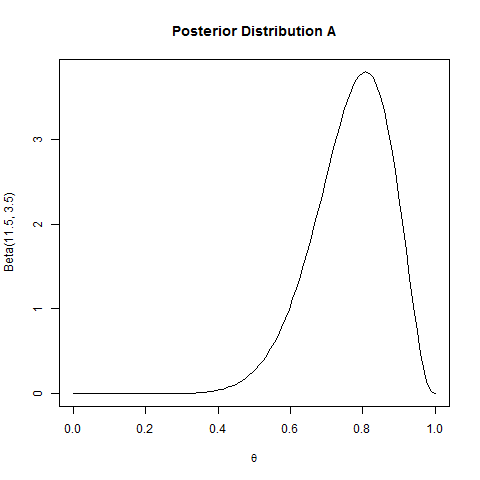
\includegraphics[scale=0.45]{densityA}
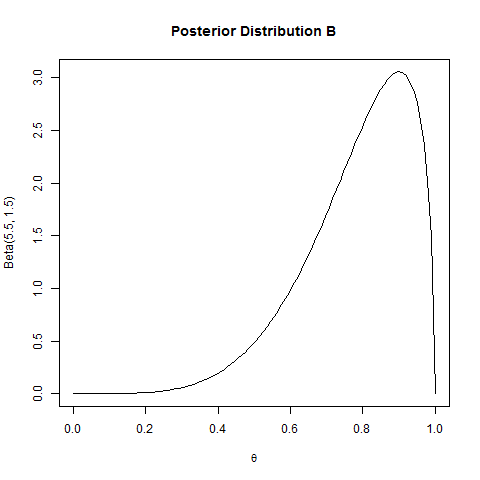
\includegraphics[scale=0.45]{densityB}

\item The probabilities that the processes are successful at least 80 \% of the time are as follows:
$$ \mathds{P}(\theta_A\geq 0.8) = 1-\mathtt{pbeta(0.8,11.5,3.5)}=0.4204$$
$$ \mathds{P}(\theta_B\geq 0.8) = 1-\mathtt{pbeta(0.8,5.5,1.5)}=0.5355$$

\item By taking large samples from posterior distributions of $\theta_A$ and $\theta_B$, the probability that solution B truly has a higher success rate than solution A is about 0.57. The exact integral to compute this probability is:
\begin{align*}
\mathds{P}(\theta_A<\theta_B|x_{A,1:n},x_{B,1:n}) & = %\int\limits_{0}^{\theta_B}\mathds{1}(\theta_A<\theta_B)p(\theta_A,\theta_B|x_{A,1:n},x_{B,1:n})d\theta_A \\
\int\limits_{0}^{1} \int\limits_{0}^{\theta_B}p(\theta_A,\theta_B|x_{A,1:n},x_{B,1:n})d\theta_A d\theta_B
\end{align*}

\item Based on the fact that the probability that solution B truly has a higher success rate than solution A is about 0.57, she should use solution B.
\end{enumerate}
See below for R code written to perform above analyses and calculations.

\listinginput[1]{1}{lab1.r}


\end{document}